\documentclass[12pt,a4paper]{article}
\usepackage[utf8]{inputenc}
\usepackage[italian]{babel}
\usepackage{geometry}
\usepackage{graphicx}
\usepackage{titlesec}
\usepackage{longtable}
\usepackage{tabularx}
\usepackage{enumitem}
\usepackage{graphicx}
\usepackage{hyperref}
\usepackage{booktabs}
\usepackage{ltablex}
\usepackage[table]{xcolor}
\graphicspath{ {./pictures/} } % definisce la cartella predefinita per le immagini
\usepackage{float}
\geometry{margin=2.5cm}

\begin{document}

% --- PAGINA 1: COPERTINA ---
\begin{titlepage}

    \centering
    \vspace*{2cm}
    {\Huge \textbf{RiciclApp} \par}
    \vspace{1cm}
    {\Large Deliverable D3 \par}
    \vspace{3cm}
    
    {\large \textbf{Gruppo n°:} 20 \par}
    \vspace{1.5cm}
    
    {\large \textbf{Componenti:} \par}
    \vspace{0.5cm}
    \begin{tabular}{rl}
        \textbf{Studente:} & Binco Francesco (Matricola: 243781) \\
        \textbf{Studente:} & Cortese Riccardo (Matricola: 244656) \\
        \textbf{Studente:} & Giovagnetti Lorenzo (Matricola: 247579) \\
    \end{tabular}
    
    \vfill
    {\large Progetto di Ingegneria del Software - Prof. Sandro Luigi Fiore \par}
    \vspace{1.5cm}
    {\large Anno Accademico 2025/2026 \par}
    \vspace{2cm}
\end{titlepage}

% --- PAGINA 2: SOMMARIO ---

\begin{abstract}

Il presente progetto descrive l'ideazione e la progettazione di un sistema per l'ottimizzazione della raccolta differenziata urbana. 

L'obiettivo principale dell'applicazione è duplice: da un lato, semplificare il conferimento dei rifiuti per il cittadino attraverso strumenti di riconoscimento (scansione barcode) e localizzazione dei punti di raccolta con relativo stato di riempimento; dall'altro, fornire agli enti comunali e alle aziende di raccolta una visione d'insieme in tempo reale dello stato del territorio. 

Grazie ai dati trasmessi dai sensori IoT installati nei bidoni, l'amministratore può monitorare i livelli di riempimento, identificare le zone critiche e pianificare interventi di svuotamento mirati. Questo approccio permette di passare da una raccolta a calendario a una gestione dinamica "on-demand", riducendo i costi operativi e l'impatto ambientale dei mezzi di trasporto. 

Il sistema si avvale di una rete di sensori IoT installati nei bidoni stradali per il monitoraggio in tempo reale dei livelli di riempimento, permettendo agli operatori ecologici di usufruire di percorsi di raccolta ottimizzati. 
\end{abstract}


% --- PAGINA 3: INDICE ---
\newpage
\pagenumbering{roman} % Numerazione romana per l'indice
\tableofcontents
\newpage
\pagenumbering{arabic}


\section{Sezione introduttiva}

\subsection{Team Memebrs}

Il team è composto da:
\begin{itemize}
    \item Binco Francesco
    \begin{itemize}
        \item Matricola: 243781
        \item Account GitHub: BincoFrancesco
    \end{itemize}
    \item Cortese Riccardo
    \begin{itemize}
        \item Matricola: 244656
        \item Account GitHub: RiccardoCortese
    \end{itemize}
    \item  Giovagnetti Lorenzo
    \begin{itemize}
        \item Matricola: 247579
        \item Account GitHub: DuduTheGreat

    \end{itemize}
\end{itemize}

\subsection{Project Idea}

Il presente progetto descrive l'ideazione e la progettazione di un sistema per l'ottimizzazione della raccolta differenziata urbana. 

L'obiettivo principale dell'applicazione è duplice: da un lato, semplificare il conferimento dei rifiuti per il cittadino attraverso strumenti di riconoscimento  e localizzazione dei punti di raccolta; dall'altro, fornire agli enti comunali e alle aziende di raccolta una visione d'insieme in tempo reale dello stato del territorio. 


\subsection{Links}

In questa sezione riportiamo i link utili al reperimento della repository e alla documentazione:

\begin{itemize}
    \item Repository GitHub: https://github.com/RiccardoCortese/RiciclApp/tree/main
    \item Swagger: https://app.swaggerhub.com/apis/uni-01b-515/RiciclApp/1.0.0
\end{itemize}

\section{Sezione generale}

\subsection{Strategia di branching adottata}

Per lo sviluppo del progetto il nostro team ha addottato la strategia di branch denominata \textit{GitFlow}.

Abbiamo fatto la seguente divisione per i branch:
\begin{itemize}
    \item \textbf{Main}: questo branch contiene solamente le realise stabili dell'applicazione
    \item \textbf{Develop}: questo è il branch principale utilizzato durante lo sviluppo. Contiene tutte le feature completate.
    \item \textbf{Branch feature}: questi branch contengono l'implementazione delle singole feature. Una volta completate viene fatto il merge nel branch \textit{Develop}
\end{itemize}

\subsection{Product Backlog}

Riportiamo il link per visualizzare il \textit{product backlog} per il nostro progetto

\textbf{Product Backlog}: \href{https://docs.google.com/spreadsheets/d/125j1VX_FSA3DJzB0BaUx1eusFmqfIbEHgwuWGOA6cfo/edit?gid=824923259#gid=824923259}{link} 

\subsection{Definizione di Done}

Per lo sviluppo del nostro progetto abbiamo utilizzato la seguente definizione di \textit{Done}:
\begin{itemize}
    \item Analisi e ricerca delle tecnologie usate
    \item Implementazione del codice
    \item Testing delle features sviluppate
    \item Documentazione (OpenAPI)
    \item Merge branch feature in branch develop
    \item Testing del branch develop
\end{itemize}

\section{Sezione sprint \#1}

\subsection{Goal}

Il goal per questo sprint era quello di creare una prima realise della nostra applicazione concentrandoci sull'implementazione delle funzionalià per un utente base.

Sono state sviluppate funzionalità come:
\begin{itemize}
    \item Registrazione;
    \item Login;
    \item Autenticazione con JWT;
    \item Gestione account;
    \item Visualizzazione della mappa con i centri di raccolta;
    \item Scannerizzazione di codice a barre e relative informazioni per il conferimento dei rifiuti.
\end{itemize}

\subsection{Sprint Planning}

Riportiamo il link per visualizzare il \textit{Sprint backlog} per il nostro progetto

\textbf{Sprint Backlog}: \href{https://docs.google.com/spreadsheets/d/125j1VX_FSA3DJzB0BaUx1eusFmqfIbEHgwuWGOA6cfo/edit?gid=1661766441#gid=1661766441}{link} 

Riportiamo inoltre il Burndown chart

\begin{figure}[H]
    \centering
    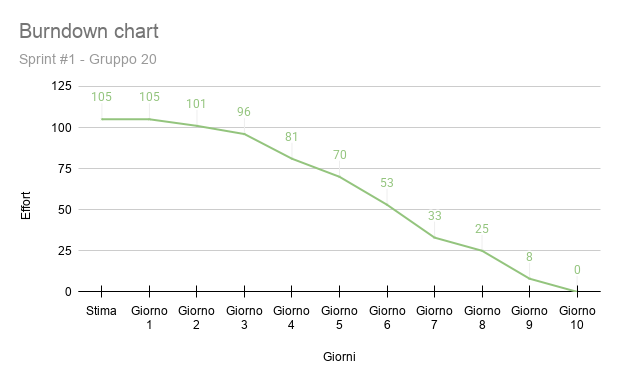
\includegraphics[width=1\linewidth]{Burndown_chart_s1.png}
    \caption{Burndown chart per sprint 1}
    \label{fig:Burndown_chart_s1}
\end{figure}

\subsection{Test cases}

iportiamo il link per visualizzare i \textit{Test cases} per il nostro progetto

\textbf{Sprint Backlog}: \href{https://docs.google.com/spreadsheets/d/125j1VX_FSA3DJzB0BaUx1eusFmqfIbEHgwuWGOA6cfo/edit?gid=1566609075#gid=1566609075}{link} 

\subsection{Product backlog refinement}

Durante uno dei meeting ci siamo accorti che il nostro prodotto potrebbe essere innovativo.

Per questo sono state apportate delle variazioni al \textit{product backlog} con aggiunta di user stories lungimiranti e che potrebbero rendere il nostro prodotto maggiormente appetibile sul mercato.

\subsection{Sprint retrospective}

Il meeting è stato molto produttivo in quanto tutti i membri del gruppo si sono dimostrati allineati per quanto riguarda gli obiettivi.  Questo ha contribuito a creare dinamiche di gruppo positive e orientate all’aiuto reciproco.

Per il prossimo sprint siamo convinti di poter aumentare la produttività, in quanto gli strumenti utilizzati per la pianificazione delle attività si sono rivelati molto utili. Inoltre, grazie a questo primo sprint, siamo riusciti a prenderne piena familiarità.

\end{document}

